\documentclass{article}
\usepackage{ifthen,libertine}
\usepackage{tikz,pgfmath,calc,xparse}
\usetikzlibrary{calc,positioning,decorations.text}
\newcommand{\myshift}{}
\begin{document}
%	\NewDocumentCommand \AlignTones {m m} {
	

	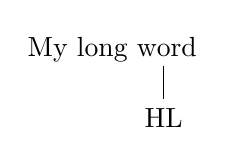
\begin{tikzpicture} [aligntones/.style={
	decorate,
	decoration={text effects along path,
		text={#1},
		text effects/.cd,
		path from text, character count=\i,
		characters={text along path,text depth=0ex,name=\i},
	    text effects={characters/.append={}}
    	},
	},
	belowcharnumber/.style={
		below=\baselineskip of #1,
		name=#1i,
		append after command={
			\pgfextra{\draw (#1.south) -- (#1i);}
		}
	}
]
	\path [aligntones=My long word] (0,0);	
%	\foreach \x/\y in {#2} {
	\node[belowcharnumber=10] {HL};
%	\draw[solid] (10) -- (10i);
		
%	\node [inner xsep=0pt,draw=red] (A) at (1,5) {Test};
%	\node [inner xsep=0pt,draw=green] (B) at (1.25,5) {Test2};
%	\path let  \p1 = ( $(A.east) - (B.west)$ ), \n1 = {veclen(\x1,\y1)} 
%	in \pgfextra{
%			\pgfmathanglebetweenpoints{\pgfpointanchor{A}{east}}{\pgfpointanchor{B}{west}}\let\abangle\pgfmathresult
%		    \pgfmathparse{or(scalar(\n1)<2.5,notequal(scalar(\abangle),0))} % 2.5pt is the width of a space in Libertine 12pt
%			\ifthenelse{\pgfmathresult=1}{\pgfmathsetlengthmacro{\myshift}{5em}}{\pgfmathsetlengthmacro{\myshift}{0pt}}
%		} node[below=of A.west,draw,xshift=\myshift,anchor=west] {\myshift \pgfmathparse{scalar(\n1)}\pgfmathresult \abangle};
	\end{tikzpicture}
%}

%\AlignTones{Nice Text!}{HL/1}
\end{document}